This chapter will introduce an approximation algorithm for the \textbf{k-anonymity with generalization} problem. The algorithm was published in 2005, in \textit{Journal of Privacy Technology}. \cite{aggarwal} The original publication is credited to the following authors: Gagan Aggarwal, Tomas Feder, Krishnaram Kenthapadi, Rajeev Motwani, Rina Panigrahy, Dilys Thomas and An Zhu.

\section{Overview}

This algorithm is a graph based algorithm. It works for any \(k\ge2\) parameter and an arbitrary alphabet size and gives an \(\mathcal{O}(k)\)-approximation solution.

The input of the algorithm is given in a form of \textit{row vectors}: \(x_1, x_2, \dots, x_n \in \Sigma^m\). Note, that the row vectors can have the same amount of components, and the corresponding elements can have the same data types, therefore representing an \(n \times m\) data table with a fixed \textit{schema}. While this is a very common use-case (and also the route we are taking with the \textbf{go implementation}) it is not necessarily required -- the algorithm could function on schema-less data.

As mentioned above, the algorithm also takes a \textit{k} integer value -- the anonymity parameter. In addition, the input also needs to contain any generalization hierarchies required to properly generalize all dimensions as specified in section \ref{sec:data_model}. In this section we will simply assume that all input is fully given and define the technicalities and possible input formats more precisely in the next chapter, when we describe the \textbf{go implementation}.

\section{Algorithm outline} \label{sec:algorithm_outline}

The outline of the algorithm can be summarized as follows:

\begin{enumerate}
    \item construct a cost-graph from the table
    \item build a forest which partitions the graph into \(c \ge k\) components
    \item gradually decompose "oversized" components until the approximation criteria is reached
\end{enumerate}

Once the last step is finished the algorithm terminates, and the output will be a \textit{forest} where each component represents a set of rows which should be generalized into the same partition.

\subsection{A note on the algorithm output}

The careful reader may notice, that the output of the above algorithm is not an anonymized data table, but a graph. If we recall the definition of \textit{k-anonymity with generalization} from section \ref{sec:definition_of_anonymity} it actually stated, that we are looking for a \textit{k-anonymous generalization function}.

Producing the generalization function from the output graph is fortunately rather straightforward. The components of the output graph tell us exactly which nodes (rows) will belong to the same partition after generalization, while the cost graph will assist us in knowing the exact level of generalization needed. Since the generalization hierarchies for each dimension were given as part of the input, the generalization function can simply be composed of applying the \textit{g} generalization function to the given level for each row vector.

Given the k-anonymous generalization function \textit{h} produced with the method above, it is a trivial matter to obtain the generalized data table: the function should be applied to each of the input data vectors: \([h(x_1), h(x_2), \dots, h(x_n)]\).

\section{Algorithm details}

\subsection{Cost-graph construction}

The very first step of the algorithm is the construction of a cost-graph. Given the input row vectors \(x_1, x_2, \dots, x_n \in \Sigma^m\) we create an edge-weighted complete graph \(G = (V,E)\). \cite{aggarwal} The vertex set \(V\) is constructed from the row vectors by mapping each row vector to a separate vertex.

Next we need to calculate the edge weight between every two vertices. The assigned weight needs to be proportional to the generalization cost of bringing the two connected nodes into the same partition.

\subsubsection{Unscaled Generalization cost}

Given two row vectors \textit{a} and \textit{b} from the input we will now define the unscaled generalization cost for each corresponding components of the vectors. Let \(h_{a,b}(j)\) refer to the lowest level of generalization for attribute \(j\) for which the \(j^{th}\) components of both \textit{a} and \textit{b} are in the same partition. \cite{aggarwal} Or in other words, the lowest level of generalization for the corresponding components, for which their generalized values are equal.

\subsubsection{Scaled Generalization cost}

If we scale down the above generalization cost for an attribute pair with the \textit{total number of levels} in the generalization hierarchy for the given attribute domain we get the scaled generalization cost. The resulting value will be in the range \([0..1]\). Assuming the total number of levels of generalization for the \(j^{th}\) attribute is \(l_j\), the scaled generalization cost can be formalized as \(h_{a,b}(j) / l_j\). \cite{aggarwal}

\subsubsection{Edge weight formula}

Using the scaled generalization cost for each component, the weight of an edge between the nodes representing \textit{a} and \textit{b} row vectors can be calculated with the following formula:
\begin{center}
	\(w(e)=\sum_{j}h_{a,b}(j)/l_j\).
\end{center}


\paragraph{Example} Consider the following example data:

\vspace{1cm}
\begin{figure}[H]
	\centering
	\small
	\begin{tabular}{|l|l|l|}
		\hline
		\textbf{Score} & \textbf{Grade} & \textbf{Gender} \\
		\hline
        4 & C- & male \\
		7 & B+ & male \\
		9 & A+ & female \\
        8 & A  & male \\
		\hline
	\end{tabular}
	\caption{Example data}
	\label{fig:unscaled_generalization_cost_example}
\end{figure}

Let's assume the domain for the \textit{score} attribute is integer numbers with bounds \([0..10)\), and that its generalization hierarchy can be represented with the following tree:

\vspace{1cm}
\begin{figure}[H]
    \centering


\tikzset{every picture/.style={line width=0.75pt}} %set default line width to 0.75pt

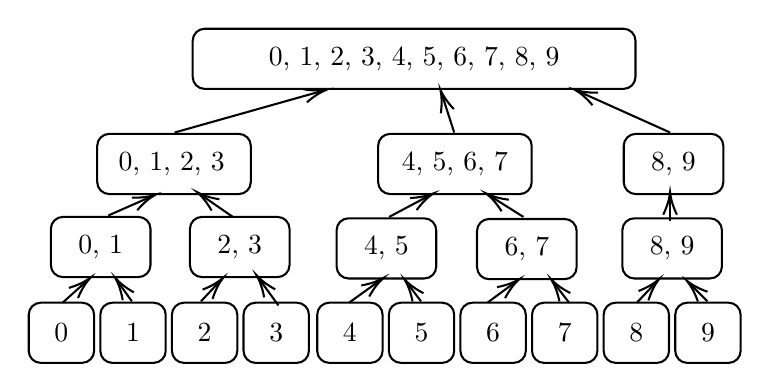
\begin{tikzpicture}[x=0.75pt,y=0.75pt,yscale=-1,xscale=1]
%uncomment if require: \path (0,457); %set diagram left start at 0, and has height of 457

%Rounded Rect [id:dp05055633926904224]
\draw   (25,105.8) .. controls (25,102.6) and (27.6,100) .. (30.8,100) -- (67.2,100) .. controls (70.4,100) and (73,102.6) .. (73,105.8) -- (73,123.2) .. controls (73,126.4) and (70.4,129) .. (67.2,129) -- (30.8,129) .. controls (27.6,129) and (25,126.4) .. (25,123.2) -- cycle ;
%Rounded Rect [id:dp14128108650523874]
\draw   (14.33,147.13) .. controls (14.33,143.93) and (16.93,141.33) .. (20.13,141.33) -- (40.03,141.33) .. controls (43.24,141.33) and (45.83,143.93) .. (45.83,147.13) -- (45.83,164.53) .. controls (45.83,167.74) and (43.24,170.33) .. (40.03,170.33) -- (20.13,170.33) .. controls (16.93,170.33) and (14.33,167.74) .. (14.33,164.53) -- cycle ;
%Rounded Rect [id:dp6850532710750563]
\draw   (48.83,147.13) .. controls (48.83,143.93) and (51.43,141.33) .. (54.63,141.33) -- (74.53,141.33) .. controls (77.74,141.33) and (80.33,143.93) .. (80.33,147.13) -- (80.33,164.53) .. controls (80.33,167.74) and (77.74,170.33) .. (74.53,170.33) -- (54.63,170.33) .. controls (51.43,170.33) and (48.83,167.74) .. (48.83,164.53) -- cycle ;
%Rounded Rect [id:dp49831794890726244]
\draw   (83.33,147.13) .. controls (83.33,143.93) and (85.93,141.33) .. (89.13,141.33) -- (109.03,141.33) .. controls (112.24,141.33) and (114.83,143.93) .. (114.83,147.13) -- (114.83,164.53) .. controls (114.83,167.74) and (112.24,170.33) .. (109.03,170.33) -- (89.13,170.33) .. controls (85.93,170.33) and (83.33,167.74) .. (83.33,164.53) -- cycle ;
%Rounded Rect [id:dp5704093284694525]
\draw   (47.33,65.8) .. controls (47.33,62.6) and (49.93,60) .. (53.13,60) -- (115.53,60) .. controls (118.74,60) and (121.33,62.6) .. (121.33,65.8) -- (121.33,83.2) .. controls (121.33,86.4) and (118.74,89) .. (115.53,89) -- (53.13,89) .. controls (49.93,89) and (47.33,86.4) .. (47.33,83.2) -- cycle ;
%Rounded Rect [id:dp06397000457352897]
\draw   (117.83,147.13) .. controls (117.83,143.93) and (120.43,141.33) .. (123.63,141.33) -- (143.53,141.33) .. controls (146.74,141.33) and (149.33,143.93) .. (149.33,147.13) -- (149.33,164.53) .. controls (149.33,167.74) and (146.74,170.33) .. (143.53,170.33) -- (123.63,170.33) .. controls (120.43,170.33) and (117.83,167.74) .. (117.83,164.53) -- cycle ;
%Rounded Rect [id:dp5625637649454729]
\draw   (153.33,147.13) .. controls (153.33,143.93) and (155.93,141.33) .. (159.13,141.33) -- (179.03,141.33) .. controls (182.24,141.33) and (184.83,143.93) .. (184.83,147.13) -- (184.83,164.53) .. controls (184.83,167.74) and (182.24,170.33) .. (179.03,170.33) -- (159.13,170.33) .. controls (155.93,170.33) and (153.33,167.74) .. (153.33,164.53) -- cycle ;
%Rounded Rect [id:dp10831678998895056]
\draw   (187.83,147.13) .. controls (187.83,143.93) and (190.43,141.33) .. (193.63,141.33) -- (213.53,141.33) .. controls (216.74,141.33) and (219.33,143.93) .. (219.33,147.13) -- (219.33,164.53) .. controls (219.33,167.74) and (216.74,170.33) .. (213.53,170.33) -- (193.63,170.33) .. controls (190.43,170.33) and (187.83,167.74) .. (187.83,164.53) -- cycle ;
%Rounded Rect [id:dp8486627726801472]
\draw   (222.33,147.13) .. controls (222.33,143.93) and (224.93,141.33) .. (228.13,141.33) -- (248.03,141.33) .. controls (251.24,141.33) and (253.83,143.93) .. (253.83,147.13) -- (253.83,164.53) .. controls (253.83,167.74) and (251.24,170.33) .. (248.03,170.33) -- (228.13,170.33) .. controls (224.93,170.33) and (222.33,167.74) .. (222.33,164.53) -- cycle ;
%Rounded Rect [id:dp16972516920971303]
\draw   (256.83,147.13) .. controls (256.83,143.93) and (259.43,141.33) .. (262.63,141.33) -- (282.53,141.33) .. controls (285.74,141.33) and (288.33,143.93) .. (288.33,147.13) -- (288.33,164.53) .. controls (288.33,167.74) and (285.74,170.33) .. (282.53,170.33) -- (262.63,170.33) .. controls (259.43,170.33) and (256.83,167.74) .. (256.83,164.53) -- cycle ;
%Rounded Rect [id:dp6840956909277642]
\draw   (291.33,147.13) .. controls (291.33,143.93) and (293.93,141.33) .. (297.13,141.33) -- (317.03,141.33) .. controls (320.24,141.33) and (322.83,143.93) .. (322.83,147.13) -- (322.83,164.53) .. controls (322.83,167.74) and (320.24,170.33) .. (317.03,170.33) -- (297.13,170.33) .. controls (293.93,170.33) and (291.33,167.74) .. (291.33,164.53) -- cycle ;
%Rounded Rect [id:dp1958758392948894]
\draw   (325.83,147.13) .. controls (325.83,143.93) and (328.43,141.33) .. (331.63,141.33) -- (351.53,141.33) .. controls (354.74,141.33) and (357.33,143.93) .. (357.33,147.13) -- (357.33,164.53) .. controls (357.33,167.74) and (354.74,170.33) .. (351.53,170.33) -- (331.63,170.33) .. controls (328.43,170.33) and (325.83,167.74) .. (325.83,164.53) -- cycle ;
%Rounded Rect [id:dp6436545397528568]
\draw   (92,105.8) .. controls (92,102.6) and (94.6,100) .. (97.8,100) -- (134.2,100) .. controls (137.4,100) and (140,102.6) .. (140,105.8) -- (140,123.2) .. controls (140,126.4) and (137.4,129) .. (134.2,129) -- (97.8,129) .. controls (94.6,129) and (92,126.4) .. (92,123.2) -- cycle ;
%Rounded Rect [id:dp3544971098617955]
\draw   (162.67,106.47) .. controls (162.67,103.26) and (165.26,100.67) .. (168.47,100.67) -- (204.87,100.67) .. controls (208.07,100.67) and (210.67,103.26) .. (210.67,106.47) -- (210.67,123.87) .. controls (210.67,127.07) and (208.07,129.67) .. (204.87,129.67) -- (168.47,129.67) .. controls (165.26,129.67) and (162.67,127.07) .. (162.67,123.87) -- cycle ;
%Rounded Rect [id:dp6212249066962128]
\draw   (230.33,106.8) .. controls (230.33,103.6) and (232.93,101) .. (236.13,101) -- (272.53,101) .. controls (275.74,101) and (278.33,103.6) .. (278.33,106.8) -- (278.33,124.2) .. controls (278.33,127.4) and (275.74,130) .. (272.53,130) -- (236.13,130) .. controls (232.93,130) and (230.33,127.4) .. (230.33,124.2) -- cycle ;
%Rounded Rect [id:dp24757598236323686]
\draw   (300.33,106.47) .. controls (300.33,103.26) and (302.93,100.67) .. (306.13,100.67) -- (342.53,100.67) .. controls (345.74,100.67) and (348.33,103.26) .. (348.33,106.47) -- (348.33,123.87) .. controls (348.33,127.07) and (345.74,129.67) .. (342.53,129.67) -- (306.13,129.67) .. controls (302.93,129.67) and (300.33,127.07) .. (300.33,123.87) -- cycle ;
%Rounded Rect [id:dp8713238483193051]
\draw   (182.67,65.8) .. controls (182.67,62.6) and (185.26,60) .. (188.47,60) -- (250.87,60) .. controls (254.07,60) and (256.67,62.6) .. (256.67,65.8) -- (256.67,83.2) .. controls (256.67,86.4) and (254.07,89) .. (250.87,89) -- (188.47,89) .. controls (185.26,89) and (182.67,86.4) .. (182.67,83.2) -- cycle ;
%Rounded Rect [id:dp8093819546801242]
\draw   (93.33,15.13) .. controls (93.33,11.93) and (95.93,9.33) .. (99.13,9.33) -- (300.87,9.33) .. controls (304.07,9.33) and (306.67,11.93) .. (306.67,15.13) -- (306.67,32.53) .. controls (306.67,35.74) and (304.07,38.33) .. (300.87,38.33) -- (99.13,38.33) .. controls (95.93,38.33) and (93.33,35.74) .. (93.33,32.53) -- cycle ;
%Rounded Rect [id:dp44931018514343335]
\draw   (301,65.8) .. controls (301,62.6) and (303.6,60) .. (306.8,60) -- (343.2,60) .. controls (346.4,60) and (349,62.6) .. (349,65.8) -- (349,83.2) .. controls (349,86.4) and (346.4,89) .. (343.2,89) -- (306.8,89) .. controls (303.6,89) and (301,86.4) .. (301,83.2) -- cycle ;
%Straight Lines [id:da27872296512255956]
\draw    (30.67,141.33) -- (42.51,130.67) ;
\draw [shift={(44,129.33)}, rotate = 498.01] [color={rgb, 255:red, 0; green, 0; blue, 0 }  ][line width=0.75]    (10.93,-3.29) .. controls (6.95,-1.4) and (3.31,-0.3) .. (0,0) .. controls (3.31,0.3) and (6.95,1.4) .. (10.93,3.29)   ;

%Straight Lines [id:da597234089010694]
\draw    (64,140.67) -- (57.15,130.97) ;
\draw [shift={(56,129.33)}, rotate = 414.78] [color={rgb, 255:red, 0; green, 0; blue, 0 }  ][line width=0.75]    (10.93,-3.29) .. controls (6.95,-1.4) and (3.31,-0.3) .. (0,0) .. controls (3.31,0.3) and (6.95,1.4) .. (10.93,3.29)   ;

%Straight Lines [id:da4850782748643834]
\draw    (97.33,140.67) -- (106.63,130.79) ;
\draw [shift={(108,129.33)}, rotate = 493.26] [color={rgb, 255:red, 0; green, 0; blue, 0 }  ][line width=0.75]    (10.93,-3.29) .. controls (6.95,-1.4) and (3.31,-0.3) .. (0,0) .. controls (3.31,0.3) and (6.95,1.4) .. (10.93,3.29)   ;

%Straight Lines [id:da7930566056169013]
\draw    (134.67,142.67) -- (125.18,129.62) ;
\draw [shift={(124,128)}, rotate = 413.97] [color={rgb, 255:red, 0; green, 0; blue, 0 }  ][line width=0.75]    (10.93,-3.29) .. controls (6.95,-1.4) and (3.31,-0.3) .. (0,0) .. controls (3.31,0.3) and (6.95,1.4) .. (10.93,3.29)   ;

%Straight Lines [id:da06697954280577867]
\draw    (168.67,141.33) -- (183.71,130.5) ;
\draw [shift={(185.33,129.33)}, rotate = 504.25] [color={rgb, 255:red, 0; green, 0; blue, 0 }  ][line width=0.75]    (10.93,-3.29) .. controls (6.95,-1.4) and (3.31,-0.3) .. (0,0) .. controls (3.31,0.3) and (6.95,1.4) .. (10.93,3.29)   ;

%Straight Lines [id:da6534079236359922]
\draw    (203.33,140.67) -- (196.53,131.6) ;
\draw [shift={(195.33,130)}, rotate = 413.13] [color={rgb, 255:red, 0; green, 0; blue, 0 }  ][line width=0.75]    (10.93,-3.29) .. controls (6.95,-1.4) and (3.31,-0.3) .. (0,0) .. controls (3.31,0.3) and (6.95,1.4) .. (10.93,3.29)   ;

%Straight Lines [id:da4482322713178277]
\draw    (235.33,141.33) -- (249.06,131.19) ;
\draw [shift={(250.67,130)}, rotate = 503.53] [color={rgb, 255:red, 0; green, 0; blue, 0 }  ][line width=0.75]    (10.93,-3.29) .. controls (6.95,-1.4) and (3.31,-0.3) .. (0,0) .. controls (3.31,0.3) and (6.95,1.4) .. (10.93,3.29)   ;

%Straight Lines [id:da16086535271258762]
\draw    (274.67,141.33) -- (267.21,131.59) ;
\draw [shift={(266,130)}, rotate = 412.59000000000003] [color={rgb, 255:red, 0; green, 0; blue, 0 }  ][line width=0.75]    (10.93,-3.29) .. controls (6.95,-1.4) and (3.31,-0.3) .. (0,0) .. controls (3.31,0.3) and (6.95,1.4) .. (10.93,3.29)   ;

%Straight Lines [id:da8935727309957442]
\draw    (307.33,141.33) -- (316.63,131.46) ;
\draw [shift={(318,130)}, rotate = 493.26] [color={rgb, 255:red, 0; green, 0; blue, 0 }  ][line width=0.75]    (10.93,-3.29) .. controls (6.95,-1.4) and (3.31,-0.3) .. (0,0) .. controls (3.31,0.3) and (6.95,1.4) .. (10.93,3.29)   ;

%Straight Lines [id:da12427188024632208]
\draw    (341.33,140.67) -- (332.75,132.08) ;
\draw [shift={(331.33,130.67)}, rotate = 405] [color={rgb, 255:red, 0; green, 0; blue, 0 }  ][line width=0.75]    (10.93,-3.29) .. controls (6.95,-1.4) and (3.31,-0.3) .. (0,0) .. controls (3.31,0.3) and (6.95,1.4) .. (10.93,3.29)   ;

%Straight Lines [id:da23222234042969503]
\draw    (52.67,99.33) -- (73.5,90.14) ;
\draw [shift={(75.33,89.33)}, rotate = 516.19] [color={rgb, 255:red, 0; green, 0; blue, 0 }  ][line width=0.75]    (10.93,-3.29) .. controls (6.95,-1.4) and (3.31,-0.3) .. (0,0) .. controls (3.31,0.3) and (6.95,1.4) .. (10.93,3.29)   ;

%Straight Lines [id:da9082685186856525]
\draw    (112.67,100) -- (96.98,89.14) ;
\draw [shift={(95.33,88)}, rotate = 394.7] [color={rgb, 255:red, 0; green, 0; blue, 0 }  ][line width=0.75]    (10.93,-3.29) .. controls (6.95,-1.4) and (3.31,-0.3) .. (0,0) .. controls (3.31,0.3) and (6.95,1.4) .. (10.93,3.29)   ;

%Straight Lines [id:da035871989319939956]
\draw    (188,100) -- (207.57,89.6) ;
\draw [shift={(209.33,88.67)}, rotate = 512.02] [color={rgb, 255:red, 0; green, 0; blue, 0 }  ][line width=0.75]    (10.93,-3.29) .. controls (6.95,-1.4) and (3.31,-0.3) .. (0,0) .. controls (3.31,0.3) and (6.95,1.4) .. (10.93,3.29)   ;

%Straight Lines [id:da9798888674185477]
\draw    (252.67,100) -- (236.36,89.73) ;
\draw [shift={(234.67,88.67)}, rotate = 392.2] [color={rgb, 255:red, 0; green, 0; blue, 0 }  ][line width=0.75]    (10.93,-3.29) .. controls (6.95,-1.4) and (3.31,-0.3) .. (0,0) .. controls (3.31,0.3) and (6.95,1.4) .. (10.93,3.29)   ;

%Straight Lines [id:da5655371856053]
\draw    (323.33,102) -- (323.33,90) ;
\draw [shift={(323.33,88)}, rotate = 450] [color={rgb, 255:red, 0; green, 0; blue, 0 }  ][line width=0.75]    (10.93,-3.29) .. controls (6.95,-1.4) and (3.31,-0.3) .. (0,0) .. controls (3.31,0.3) and (6.95,1.4) .. (10.93,3.29)   ;

%Straight Lines [id:da5307091955398382]
\draw    (84.67,59.33) -- (156.07,39.21) ;
\draw [shift={(158,38.67)}, rotate = 524.26] [color={rgb, 255:red, 0; green, 0; blue, 0 }  ][line width=0.75]    (10.93,-3.29) .. controls (6.95,-1.4) and (3.31,-0.3) .. (0,0) .. controls (3.31,0.3) and (6.95,1.4) .. (10.93,3.29)   ;

%Straight Lines [id:da23705174012369667]
\draw    (219.33,59.33) -- (213.28,40.57) ;
\draw [shift={(212.67,38.67)}, rotate = 432.12] [color={rgb, 255:red, 0; green, 0; blue, 0 }  ][line width=0.75]    (10.93,-3.29) .. controls (6.95,-1.4) and (3.31,-0.3) .. (0,0) .. controls (3.31,0.3) and (6.95,1.4) .. (10.93,3.29)   ;

%Straight Lines [id:da10111862824392315]
\draw    (323.33,59.33) -- (279.16,39.49) ;
\draw [shift={(277.33,38.67)}, rotate = 384.19] [color={rgb, 255:red, 0; green, 0; blue, 0 }  ][line width=0.75]    (10.93,-3.29) .. controls (6.95,-1.4) and (3.31,-0.3) .. (0,0) .. controls (3.31,0.3) and (6.95,1.4) .. (10.93,3.29)   ;


% Text Node
\draw (30.08,155.83) node  [align=left] {0};
% Text Node
\draw (64.58,155.83) node  [align=left] {1};
% Text Node
\draw (99.08,155.83) node  [align=left] {2};
% Text Node
\draw (133.58,155.83) node  [align=left] {3};
% Text Node
\draw (169.08,155.83) node  [align=left] {4};
% Text Node
\draw (203.58,155.83) node  [align=left] {5};
% Text Node
\draw (238.08,155.83) node  [align=left] {6};
% Text Node
\draw (272.58,155.83) node  [align=left] {7};
% Text Node
\draw (307.08,155.83) node  [align=left] {8};
% Text Node
\draw (341.58,155.83) node  [align=left] {9};
% Text Node
\draw (49,114.5) node  [align=left] {0, 1};
% Text Node
\draw (116,114.5) node  [align=left] {2, 3};
% Text Node
\draw (186.67,115.17) node  [align=left] {4, 5};
% Text Node
\draw (254.33,115.5) node  [align=left] {6, 7};
% Text Node
\draw (324.33,115.17) node  [align=left] {8, 9};
% Text Node
\draw (83.17,74.5) node  [align=left] {0, 1, 2, 3};
% Text Node
\draw (219.67,74.5) node  [align=left] {4, 5, 6, 7};
% Text Node
\draw (200,23.83) node  [align=left] {0, 1, 2, 3, 4, 5, 6, 7, 8, 9};
% Text Node
\draw (325,74.5) node  [align=left] {8, 9};


\end{tikzpicture}

    \caption{Hierarchy for the score attribute}
    \label{fig:score_hierarchy}
\end{figure}

This is a valid generalization hierarchy, because each partition at the leaf nodes contain only a single element, the top level contains a single set with all elements and finally the union of all sets on every level of the hierarchy is equal to the full domain of values.

Let's calculate the generalization cost for the first two rows.

In order to transform the values of the first attribute pair \((4, 7)\) into the same partition, they need to be generalized exactly two times until their values become [4, 5, 6, 7]. This means, that the unscaled generalization cost for the score attribute \(h_{a,b}(0)=2\). The scaling factor corresponds to the highest level in the hierarchy: \(l_0=3\), so the scaled generalization cost will be \(h_{a,b}(0)/l_0=2/3\).

The edge cost between the nodes representing the first two rows will be the sum of the scaled generalization costs of \((4, 7)\), \((C-,B+)\) and \((male, male)\). Using the grade hierarchy introduced in chapter \ref{sec:data_model} in figure \ref{fig:grades-hierarchy} and considering that the values of the gender attribute are already in the same partition, so their generalization cost will be 0:
\begin{center}
	\(w(e_{a,b})=2/3+1+0=5/3\).
\end{center}


If we repeat the above calculation for each row pair, we can determine the cost-graph for this table. This process is left to the reader, but after finishing it the resulting graph should be isomorph to the graph on figure \ref{fig:cost_graph}.

\vspace{\baselineskip}
\begin{figure}[H]

\centering
\tikzset{every picture/.style={line width=0.75pt}} %set default line width to 0.75pt

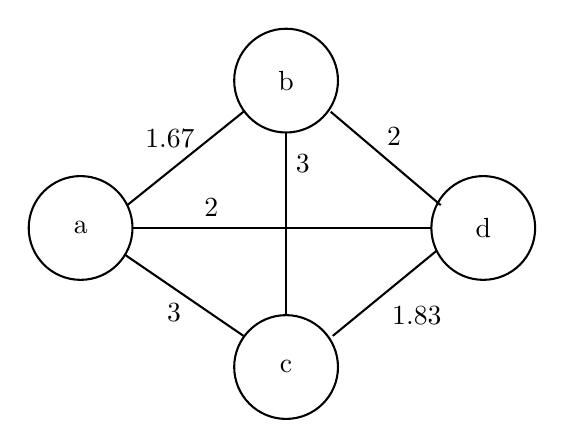
\begin{tikzpicture}[x=0.75pt,y=0.75pt,yscale=-1,xscale=1]
%uncomment if require: \path (0,300); %set diagram left start at 0, and has height of 300

%Shape: Circle [id:dp14719016101017623]
\draw   (111,126) .. controls (111,112.19) and (122.19,101) .. (136,101) .. controls (149.81,101) and (161,112.19) .. (161,126) .. controls (161,139.81) and (149.81,151) .. (136,151) .. controls (122.19,151) and (111,139.81) .. (111,126) -- cycle ;
%Shape: Circle [id:dp637969227645387]
\draw   (210,55) .. controls (210,41.19) and (221.19,30) .. (235,30) .. controls (248.81,30) and (260,41.19) .. (260,55) .. controls (260,68.81) and (248.81,80) .. (235,80) .. controls (221.19,80) and (210,68.81) .. (210,55) -- cycle ;
%Shape: Circle [id:dp16996306115691606]
\draw   (210,193) .. controls (210,179.19) and (221.19,168) .. (235,168) .. controls (248.81,168) and (260,179.19) .. (260,193) .. controls (260,206.81) and (248.81,218) .. (235,218) .. controls (221.19,218) and (210,206.81) .. (210,193) -- cycle ;
%Shape: Circle [id:dp4723269788902422]
\draw   (305,126) .. controls (305,112.19) and (316.19,101) .. (330,101) .. controls (343.81,101) and (355,112.19) .. (355,126) .. controls (355,139.81) and (343.81,151) .. (330,151) .. controls (316.19,151) and (305,139.81) .. (305,126) -- cycle ;
%Straight Lines [id:da43115389914855107]
\draw    (158.5,115) -- (214.5,70) ;


%Straight Lines [id:da3262134359528708]
\draw    (257.5,178) -- (307.5,137) ;


%Straight Lines [id:da6644861489456326]
\draw    (235,168) -- (235,80) ;


%Straight Lines [id:da44726258546505226]
\draw    (157.5,139) -- (214.5,178) ;


%Straight Lines [id:da17516578825824003]
\draw    (309.5,115) -- (256.5,70) ;


%Straight Lines [id:da25861424028019475]
\draw    (161,126) -- (305,126) ;



% Text Node
\draw (136,126) node  [align=left] {a};
% Text Node
\draw (235,55) node  [align=left] {b};
% Text Node
\draw (235,193) node  [align=left] {c};
% Text Node
\draw (330,126) node  [align=left] {d};
% Text Node
\draw (179,83) node  [align=left] {1.67};
% Text Node
\draw (181,167) node  [align=left] {3};
% Text Node
\draw (199,116) node  [align=left] {2};
% Text Node
\draw (243,95) node  [align=left] {3};
% Text Node
\draw (287,82) node  [align=left] {2};
% Text Node
\draw (298,168) node  [align=left] {1.83};


\end{tikzpicture}

	\caption{Example cost-graph}
	\label{fig:cost_graph}
\end{figure}

\subsection{A note on the limitations of the graph representation}

Unfortunately the graph representation has some limitations, as the original authors also note in their article. \cite{aggarwal} When the input data table is transformed into its graph equivalent, some information is lost which results in the algorithm only being able to achieve the \(\mathcal{O}(k)\) approximation factor.

This can be demonstrated by constructing two input tables on a binary alphabet (\(\Sigma={0,1}\)) for a given \textit{k} value in a way, that the optimal anonymization cost and the total cost incurred by the graph representation differs by a factor of \(\mathcal{O}(k)\):

Let \(l=2^{k-2}\).

\paragraph{Table A} should be \(k \times kl\), and for each row \textit{i} contains the value \textbf{1} in positions \([(i-1)l+1 \dots il]\) and \textbf{0} otherwise . The anonymization cost for this table is \(k^2l\).

\vspace{\baselineskip}
\begin{figure}[H]
	\centering
	\(
	\begin{pmatrix}
		1 & 1 & 0 & 0 & 0 & 0 \\
		0 & 0 & 1 & 1 & 0 & 0 \\
		0 & 0 & 0 & 0 & 1 & 1
	\end{pmatrix}
	\)
	\caption{Example for type A table and k=3, l=2}
	\label{fig:graph_limit_A}
\end{figure}



\paragraph{Table B} should be \(k \times 4l\). Its \(i^{th}\) row is broken down into \(2^i\) equal-sized blocks. Every value in odd blocks is \textbf{0}, and every value in even blocks is \textbf{1}. The anonymization cost for this table is \(4kl\).

\vspace{\baselineskip}
\begin{figure}[H]
	\centering
	\(
	\begin{pmatrix}
		0 & 0 & 0 & 0 & 1 & 1 & 1 & 1 \\
		0 & 0 & 1 & 1 & 0 & 0 & 1 & 1 \\
		0 & 1 & 0 & 1 & 0 & 1 & 0 & 1
	\end{pmatrix}
	\)
	\caption{Example for type B table and k=3, l=2}
	\label{fig:graph_limit_B}
\end{figure}

Note, that both tables are represented by a k-clique with all edge costs being \(2l=2^{k-1}\), while their respective anonymization cost differs by exactly \(\mathcal{O}(k)\).

\vspace{\baselineskip}
\begin{figure}[H]
	\centering


\tikzset{every picture/.style={line width=0.75pt}} %set default line width to 0.75pt

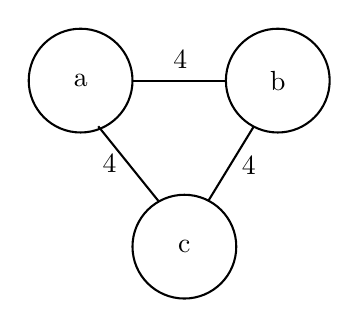
\begin{tikzpicture}[x=0.75pt,y=0.75pt,yscale=-1,xscale=1]
%uncomment if require: \path (0,300); %set diagram left start at 0, and has height of 300

%Shape: Circle [id:dp058849468526875004]
\draw   (59,60) .. controls (59,46.19) and (70.19,35) .. (84,35) .. controls (97.81,35) and (109,46.19) .. (109,60) .. controls (109,73.81) and (97.81,85) .. (84,85) .. controls (70.19,85) and (59,73.81) .. (59,60) -- cycle ;
%Shape: Circle [id:dp11003911798399524]
\draw   (154,60) .. controls (154,46.19) and (165.19,35) .. (179,35) .. controls (192.81,35) and (204,46.19) .. (204,60) .. controls (204,73.81) and (192.81,85) .. (179,85) .. controls (165.19,85) and (154,73.81) .. (154,60) -- cycle ;
%Shape: Circle [id:dp7927588085940704]
\draw   (109,140) .. controls (109,126.19) and (120.19,115) .. (134,115) .. controls (147.81,115) and (159,126.19) .. (159,140) .. controls (159,153.81) and (147.81,165) .. (134,165) .. controls (120.19,165) and (109,153.81) .. (109,140) -- cycle ;
%Straight Lines [id:da30216407066666995]
\draw    (109,60) -- (154,60) ;


%Straight Lines [id:da024128079077286868]
\draw    (92.5,82) -- (121.5,118) ;


%Straight Lines [id:da48310889364666654]
\draw    (167.5,82) -- (145.5,118) ;



% Text Node
\draw (84,60) node  [align=left] {a};
% Text Node
\draw (179,60) node  [align=left] {b};
% Text Node
\draw (134,140) node  [align=left] {c};
% Text Node
\draw (132,50) node  [align=left] {4};
% Text Node
\draw (98,100) node  [align=left] {4};
% Text Node
\draw (165,101) node  [align=left] {4};


\end{tikzpicture}

	\caption{Graph representation of both Table A and Table B}
	\label{fig:graph_limit_graph}

\end{figure}

\subsection{Forest building algorithm}

The next step in the overall k-anonymity algorithm is to produce a forest. (Section \ref{sec:algorithm_outline}) We will now use the nodes and calculated weights from the cost-graph, but in this step we will be constructing a directed graph which will ultimately be used to represent a partitioning of the original row vectors.

\paragraph{Algorithm} \textsc{Forest building} \cite{aggarwal}

Invariant:
\begin{itemize}
	\item The chosen edges do not create any cycle.
	\item The out-degree of each vertex is at most one.
\end{itemize}

Steps:
\begin{enumerate}
	\item Start with an empty edge set so that each vertex is in its own connected component.
	\item Repeat until all components are of size at least \textit{k}: \par
	Pick any component \textit{T} having size smaller than \textit{k}. Let \textit{u} be a vertex in \textit{T} without any outgoing edges. Since there are at most \(k-2\) other vertices in \textit{T}, one of the \(k-1\) \emph{nearest neighbors} of \textit{u}, say \textit{v}, must lie outside \textit{T}. We add the edge \(\vec{uv}\) to the forest. \textit{(Observe that this step does not violate any of the invariants.)}
\end{enumerate}

\vspace{\baselineskip}

In simple terms we start from the original graph without any edges. In every step we extend a selected tree (\(size < k\)) in the forest. We add a new vertex to the tree by selecting an \textit{u} "leaf" (without any outgoing edges) in the current tree, and connecting it with its lowest cost neighbor \textit{v}.

\paragraph{Lemma} The forest produced by the Forest building algorithm has a minimum tree size at least \textit{k} and has cost at most \textit{OPT}, where \textit{OPT} denotes the cost of an optimal k-anonymity solution. \cite{aggarwal}

\paragraph{Example} Forest building (\(k=3\)) \label{sec:forest_building_example}

For this example let's assume that the cost-graph has already been computed from the input table, and is isomorph to the graph shown on figure \ref{fig:forest_cost_graph}.

\vspace{\baselineskip}
\begin{figure}[H]
	\centering
	\includegraphics[width=200pt]{../graphs/forest-example-cost.png}
	\caption{Example cost graph}
	\label{fig:forest_cost_graph}
\end{figure}

The starting position has all nodes in their separate component. From there, the steps of the algorithm can be traced on figure \ref{fig:forest_partitioning}.

\begin{figure}
	\centering
	\subfloat[Step 1]{{\includegraphics[width=6cm]{../graphs/forest-example-1.png} }}
    \vspace{0.6cm}
	\subfloat[Step 2]{{\includegraphics[width=6cm]{../graphs/forest-example-2.png} }}
	\vspace{0.6cm}
	\subfloat[Step 3]{{\includegraphics[width=6cm]{../graphs/forest-example-3.png} }}
	\vspace{0.6cm}
	\subfloat[Step 4]{{\includegraphics[width=6cm]{../graphs/forest-example-4.png} }}
	\vspace{0.6cm}
	\subfloat[Step 5]{{\includegraphics[width=6cm]{../graphs/forest-example-5.png} }}
	\vspace{0.6cm}
    \subfloat[Step 6]{{\includegraphics[width=6cm]{../graphs/forest-example-6.png} }}
    \caption{Forest Building Algorithm}
    \label{fig:forest_partitioning}
\end{figure}

The forest building algorithm starts from an empty edge set. Each node is in a separate component. Since at this point the size of each component is smaller than \textit{k}, we pick a component to extend at random.

In Step 1 of the example we picked the component which contains the \textit{c} node. Inspecting the outgoing edges we find that the closest one is the edge going to \textit{b}. In Step 2 we continue extending the same component, since its size is still under the threshold. Node \textit{b} is now part of the component, and has no outgoing edges, so we try to find an outgoing edge from that. Closest is the component containing \textit{e}, so we add it.

At this point, the component's size has reached \(k=3\), so we move on to another component to extend. In Step 4 we have picked \textit{d}. Note, at this point when considering the possible edges we also considered edges between \textit{d} and nodes in the previously created component (\textit{b} and \textit{e}). This is an example of how this part of the algorithm could end up with component sizes greater than \textit{k}. In this example however, the closest neighbor is \textit{f}, and by Step 6 we can cleanly finish the partitioning with two 3-node partitions.

\subsection{Algorithm to decompose oversized components}

In the example in section \ref{sec:forest_building_example} we fortunately ended up with two perfectly sized components, which defined a good partitioning for anonymization. This will not always be the case however, and there may be oversized components in the forest.

In this section we show an algorithm to break any component with size \(s \ge max\{2k-1, 3k-5\}\) into two components each of size at least \textit{k}. (The following algorithm treats the component as an \emph{undirected} graph.)

\paragraph{Algorithm} \textsc{Decompose component} \cite{aggarwal}

\begin{enumerate}
	\item Pick any vertex \textit{u} as the candidate vertex.
	\item Root the tree at the candidate vertex \textit{u}. Let U be the set of subtrees rooted at the children of \textit{u}. Let the size of the largest subtree of \textit{u} be \(\phi\), rooted at vertex \textit{v}. (See figure \ref{fig:decompose}) If \(s-\phi \ge k-1\), then we do one of the following partition and terminate:
	\begin{enumerate}
		\item[A)] If \(\phi \ge k\) and \(s-\phi \ge k\), then partition the tree into the largest subtree and the rest.
		\item[B)] If \(s-\phi = k-1\), partition the tree into a component containing the subtrees rooted at the children of \textit{v} and the rest. To connect the children of \textit{v} create a \emph{Steiner's Vertex} (see below).
		\item[C)] If \(\phi = k-1\), then partition into a component containing the subtree rooted at \textit{v} along with the vertex \textit{u} and the rest. In order to connect the children of \textit{u} create a \emph{Steiner's Vertex}.
		\item[D)] Otherwise, all subtrees have size at most \(k-2\). In this case, we create an empty partition and keep adding subtrees of \textit{u} to it until the first time its size becomes at least \(k-1\). Put the remaining subtrees into the other partition. If one of the partitions has size equal to \(k-1\), add \textit{u} to that partition. Otherwise add \textit{u} to the first partition. In the partition not containing \textit{u} add a \emph{Steiner's Vertex} to keep it connected.
	\end{enumerate}
	\item Otherwise, pick \textit{v} as the new candidate vertex and go to Step 2.
\end{enumerate}

\vspace{\baselineskip}
\begin{figure}[H]
	\centering


\tikzset{every picture/.style={line width=0.75pt}} %set default line width to 0.75pt

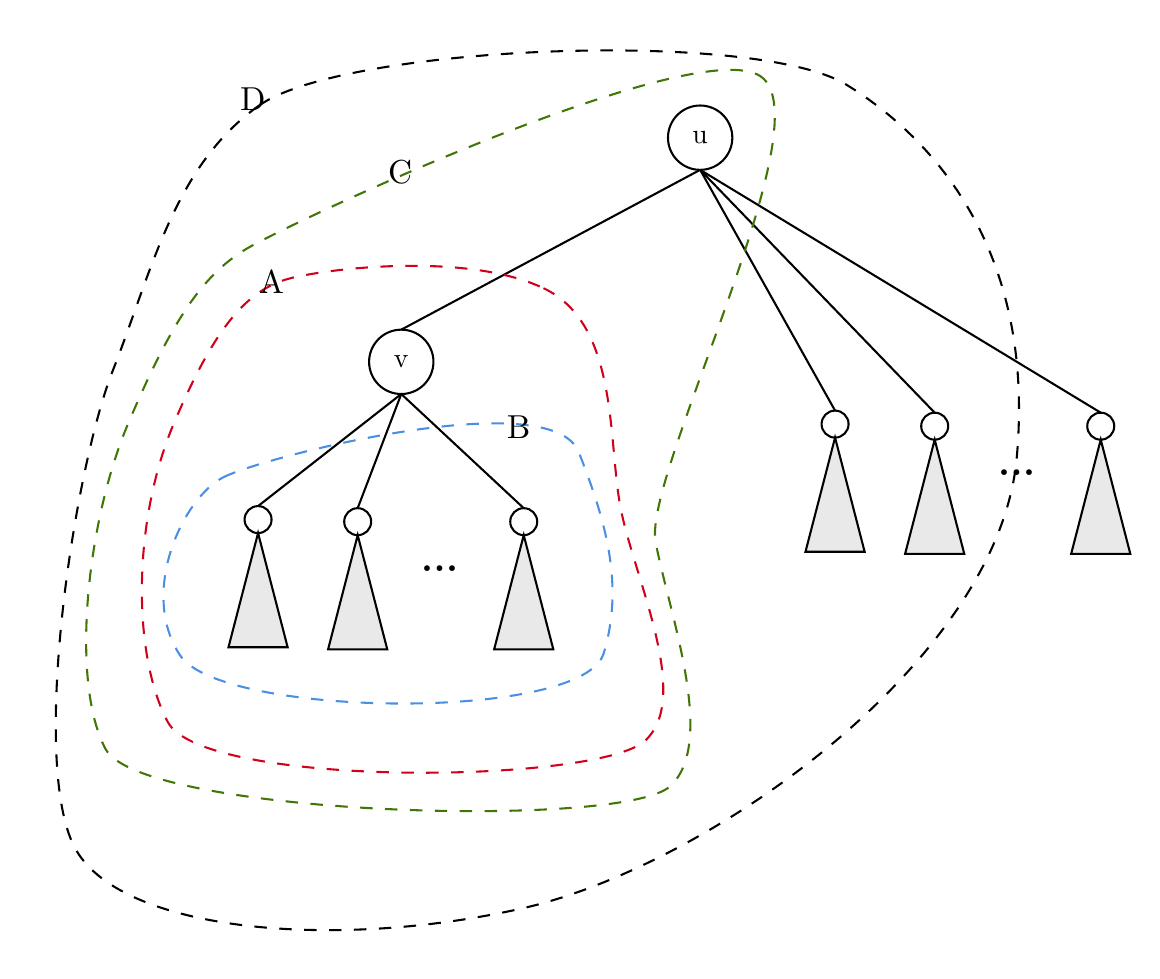
\begin{tikzpicture}[x=0.75pt,y=0.75pt,yscale=-1,xscale=1]
%uncomment if require: \path (0,459); %set diagram left start at 0, and has height of 459

%Shape: Circle [id:dp7711684678996311]
\draw  [fill={rgb, 255:red, 255; green, 255; blue, 255 }  ,fill opacity=1 ] (302,48.5) .. controls (302,39.94) and (308.94,33) .. (317.5,33) .. controls (326.06,33) and (333,39.94) .. (333,48.5) .. controls (333,57.06) and (326.06,64) .. (317.5,64) .. controls (308.94,64) and (302,57.06) .. (302,48.5) -- cycle ;
%Shape: Circle [id:dp8540052293183187]
\draw  [fill={rgb, 255:red, 255; green, 255; blue, 255 }  ,fill opacity=1 ] (158,156.5) .. controls (158,147.94) and (164.94,141) .. (173.5,141) .. controls (182.06,141) and (189,147.94) .. (189,156.5) .. controls (189,165.06) and (182.06,172) .. (173.5,172) .. controls (164.94,172) and (158,165.06) .. (158,156.5) -- cycle ;
%Shape: Circle [id:dp6767312206403671]
\draw   (98,232.5) .. controls (98,228.91) and (100.91,226) .. (104.5,226) .. controls (108.09,226) and (111,228.91) .. (111,232.5) .. controls (111,236.09) and (108.09,239) .. (104.5,239) .. controls (100.91,239) and (98,236.09) .. (98,232.5) -- cycle ;
%Shape: Triangle [id:dp6284155562718452]
\draw  [fill={rgb, 255:red, 233; green, 233; blue, 233 }  ,fill opacity=1 ] (104.5,239) -- (118.75,294) -- (90.25,294) -- cycle ;
%Shape: Circle [id:dp024913106678187136]
\draw   (146,233.5) .. controls (146,229.91) and (148.91,227) .. (152.5,227) .. controls (156.09,227) and (159,229.91) .. (159,233.5) .. controls (159,237.09) and (156.09,240) .. (152.5,240) .. controls (148.91,240) and (146,237.09) .. (146,233.5) -- cycle ;
%Shape: Triangle [id:dp11973699329342047]
\draw  [fill={rgb, 255:red, 233; green, 233; blue, 233 }  ,fill opacity=1 ] (152.5,240) -- (166.75,295) -- (138.25,295) -- cycle ;
%Shape: Circle [id:dp5828391286835717]
\draw   (226,233.5) .. controls (226,229.91) and (228.91,227) .. (232.5,227) .. controls (236.09,227) and (239,229.91) .. (239,233.5) .. controls (239,237.09) and (236.09,240) .. (232.5,240) .. controls (228.91,240) and (226,237.09) .. (226,233.5) -- cycle ;
%Shape: Triangle [id:dp2511681856589991]
\draw  [fill={rgb, 255:red, 233; green, 233; blue, 233 }  ,fill opacity=1 ] (232.5,240) -- (246.75,295) -- (218.25,295) -- cycle ;
%Shape: Circle [id:dp5623627355443772]
\draw   (376,186.5) .. controls (376,182.91) and (378.91,180) .. (382.5,180) .. controls (386.09,180) and (389,182.91) .. (389,186.5) .. controls (389,190.09) and (386.09,193) .. (382.5,193) .. controls (378.91,193) and (376,190.09) .. (376,186.5) -- cycle ;
%Shape: Triangle [id:dp39244508786141674]
\draw  [fill={rgb, 255:red, 233; green, 233; blue, 233 }  ,fill opacity=1 ] (382.5,193) -- (396.75,248) -- (368.25,248) -- cycle ;
%Shape: Circle [id:dp8178713595847904]
\draw   (424,187.5) .. controls (424,183.91) and (426.91,181) .. (430.5,181) .. controls (434.09,181) and (437,183.91) .. (437,187.5) .. controls (437,191.09) and (434.09,194) .. (430.5,194) .. controls (426.91,194) and (424,191.09) .. (424,187.5) -- cycle ;
%Shape: Triangle [id:dp3542102499533475]
\draw  [fill={rgb, 255:red, 233; green, 233; blue, 233 }  ,fill opacity=1 ] (430.5,194) -- (444.75,249) -- (416.25,249) -- cycle ;
%Shape: Circle [id:dp4483381477394748]
\draw   (504,187.5) .. controls (504,183.91) and (506.91,181) .. (510.5,181) .. controls (514.09,181) and (517,183.91) .. (517,187.5) .. controls (517,191.09) and (514.09,194) .. (510.5,194) .. controls (506.91,194) and (504,191.09) .. (504,187.5) -- cycle ;
%Shape: Triangle [id:dp4240387998981314]
\draw  [fill={rgb, 255:red, 233; green, 233; blue, 233 }  ,fill opacity=1 ] (510.5,194) -- (524.75,249) -- (496.25,249) -- cycle ;
%Straight Lines [id:da29060880873239037]
\draw    (317.5,64) -- (173.5,141) ;


%Straight Lines [id:da681996043601955]
\draw    (317.5,64) -- (382.5,180) ;


%Straight Lines [id:da7335165640252448]
\draw    (317.5,64) -- (430.5,181) ;


%Straight Lines [id:da39989551498039266]
\draw    (317.5,64) -- (510.5,181) ;


%Straight Lines [id:da27519719998677683]
\draw    (104.5,226) -- (173.5,172) ;


%Straight Lines [id:da1425001048459873]
\draw    (152.5,227) -- (173.5,172) ;


%Straight Lines [id:da8004516890426716]
\draw    (232.5,227) -- (173.5,172) ;


%Shape: Polygon Curved [id:ds10919181429761804]
\draw  [color={rgb, 255:red, 208; green, 2; blue, 27 }  ,draw opacity=1 ][dash pattern={on 4.5pt off 4.5pt}] (242,121) .. controls (278,138) and (273,193) .. (279,226) .. controls (285,259) and (314,318) .. (291,339) .. controls (268,360) and (78,362) .. (61,330) .. controls (44,298) and (43.75,233.63) .. (64,186) .. controls (84.25,138.38) and (100,121) .. (121,116) .. controls (142,111) and (206,104) .. (242,121) -- cycle ;
%Shape: Polygon Curved [id:ds3630985664957256]
\draw  [color={rgb, 255:red, 74; green, 144; blue, 226 }  ,draw opacity=1 ][dash pattern={on 4.5pt off 4.5pt}] (88,212) .. controls (108,202) and (246,167) .. (259,200) .. controls (272,233) and (281,264) .. (271,297) .. controls (261,330) and (87,328) .. (67,298) .. controls (47,268) and (68,222) .. (88,212) -- cycle ;
%Shape: Polygon Curved [id:ds6625985709394309]
\draw  [color={rgb, 255:red, 65; green, 117; blue, 5 }  ,draw opacity=1 ][dash pattern={on 4.5pt off 4.5pt}] (345,18) .. controls (381,35) and (290,210) .. (296,243) .. controls (302,276) and (326,340) .. (303,361) .. controls (280,382) and (48,375) .. (31,343) .. controls (14,311) and (21.75,233.63) .. (42,186) .. controls (62.25,138.38) and (77,115) .. (99,102) .. controls (121,89) and (309,1) .. (345,18) -- cycle ;
%Shape: Polygon Curved [id:ds5228551783856155]
\draw  [color={rgb, 255:red, 0; green, 0; blue, 0 }  ,draw opacity=1 ][dash pattern={on 4.5pt off 4.5pt}] (105,33) .. controls (146,4) and (344,-4) .. (388,23) .. controls (432,50) and (479,105) .. (470,203) .. controls (461,301) and (321,400) .. (231,420) .. controls (141,440) and (40,431) .. (17,392) .. controls (-6,353) and (15.5,209) .. (34.5,160.75) .. controls (53.5,112.5) and (64,62) .. (105,33) -- cycle ;

% Text Node
\draw (317.5,48.5) node  [align=left] {u};
% Text Node
\draw (173.5,156.5) node  [align=left] {v};
% Text Node
\draw (192,256) node  [align=left] {\textbf{{\Large ...}}};
% Text Node
\draw (470,210) node  [align=left] {\textbf{{\Large ...}}};
% Text Node
\draw (111,118) node [scale=1.2] [align=left] {A};
% Text Node
\draw (230,188) node [scale=1.2] [align=left] {B};
% Text Node
\draw (173,65) node [scale=1.2] [align=left] {C};
% Text Node
\draw (102,30) node [scale=1.2] [align=left] {D};


\end{tikzpicture}

	\caption{Different cut types for the decompose algorithm}
	\label{fig:decompose}
\end{figure}

\paragraph{The Steiner's Vertex} is a dummy vertex inserted to structurally hold the component together, but does not contribute to the size of the component during the algorithm.

\vspace{\baselineskip}
\begin{figure}[H]
	\centering




	\tikzset{every picture/.style={line width=0.75pt}} %set default line width to 0.75pt

	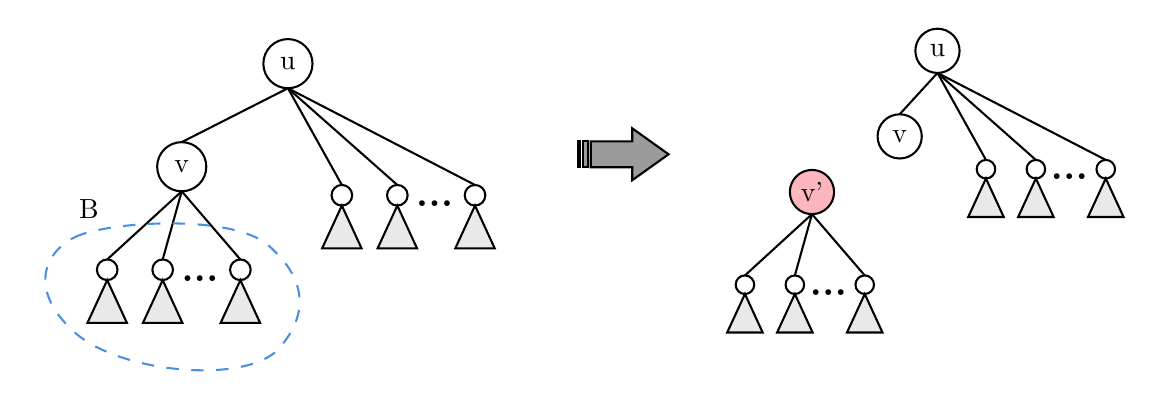
\begin{tikzpicture}[x=0.75pt,y=0.75pt,yscale=-1,xscale=1]
	%uncomment if require: \path (0,476); %set diagram left start at 0, and has height of 476

	%Shape: Ellipse [id:dp7890393065744103]
	\draw  [fill={rgb, 255:red, 255; green, 255; blue, 255 }  ,fill opacity=1 ] (124.52,36.84) .. controls (124.52,30.3) and (129.83,25) .. (136.36,25) .. controls (142.9,25) and (148.2,30.3) .. (148.2,36.84) .. controls (148.2,43.38) and (142.9,48.68) .. (136.36,48.68) .. controls (129.83,48.68) and (124.52,43.38) .. (124.52,36.84) -- cycle ;
	%Shape: Ellipse [id:dp618735643725828]
	\draw  [fill={rgb, 255:red, 255; green, 255; blue, 255 }  ,fill opacity=1 ] (73.35,86.49) .. controls (73.35,79.95) and (78.65,74.65) .. (85.19,74.65) .. controls (91.72,74.65) and (97.03,79.95) .. (97.03,86.49) .. controls (97.03,93.03) and (91.72,98.33) .. (85.19,98.33) .. controls (78.65,98.33) and (73.35,93.03) .. (73.35,86.49) -- cycle ;
	%Shape: Ellipse [id:dp4771904397826303]
	\draw   (44.32,136.14) .. controls (44.32,133.4) and (46.54,131.18) .. (49.28,131.18) .. controls (52.03,131.18) and (54.25,133.4) .. (54.25,136.14) .. controls (54.25,138.88) and (52.03,141.11) .. (49.28,141.11) .. controls (46.54,141.11) and (44.32,138.88) .. (44.32,136.14) -- cycle ;
	%Shape: Triangle [id:dp553752456661303]
	\draw  [fill={rgb, 255:red, 233; green, 233; blue, 233 }  ,fill opacity=1 ] (49.28,141.11) -- (58.78,161.73) -- (39.78,161.73) -- cycle ;

	%Shape: Ellipse [id:dp4582325504788667]
	\draw   (71.05,136.14) .. controls (71.05,133.4) and (73.28,131.18) .. (76.02,131.18) .. controls (78.76,131.18) and (80.98,133.4) .. (80.98,136.14) .. controls (80.98,138.88) and (78.76,141.11) .. (76.02,141.11) .. controls (73.28,141.11) and (71.05,138.88) .. (71.05,136.14) -- cycle ;
	%Shape: Triangle [id:dp5979831512805434]
	\draw  [fill={rgb, 255:red, 233; green, 233; blue, 233 }  ,fill opacity=1 ] (76.02,141.11) -- (85.52,161.73) -- (66.52,161.73) -- cycle ;

	%Shape: Ellipse [id:dp2963506198722945]
	\draw   (108.48,136.14) .. controls (108.48,133.4) and (110.71,131.18) .. (113.45,131.18) .. controls (116.19,131.18) and (118.41,133.4) .. (118.41,136.14) .. controls (118.41,138.88) and (116.19,141.11) .. (113.45,141.11) .. controls (110.71,141.11) and (108.48,138.88) .. (108.48,136.14) -- cycle ;
	%Shape: Triangle [id:dp6725407515322526]
	\draw  [fill={rgb, 255:red, 233; green, 233; blue, 233 }  ,fill opacity=1 ] (113.45,141.11) -- (122.95,161.73) -- (103.95,161.73) -- cycle ;

	%Shape: Circle [id:dp18476563967542958]
	\draw   (157.37,100.24) .. controls (157.37,97.5) and (159.59,95.28) .. (162.34,95.28) .. controls (165.08,95.28) and (167.3,97.5) .. (167.3,100.24) .. controls (167.3,102.98) and (165.08,105.21) .. (162.34,105.21) .. controls (159.59,105.21) and (157.37,102.98) .. (157.37,100.24) -- cycle ;
	%Shape: Triangle [id:dp466803100468395]
	\draw  [fill={rgb, 255:red, 233; green, 233; blue, 233 }  ,fill opacity=1 ] (162.34,105.21) -- (171.84,125.83) -- (152.83,125.83) -- cycle ;

	%Shape: Circle [id:dp5261729680381961]
	\draw   (184.11,100.24) .. controls (184.11,97.5) and (186.33,95.28) .. (189.07,95.28) .. controls (191.81,95.28) and (194.04,97.5) .. (194.04,100.24) .. controls (194.04,102.98) and (191.81,105.21) .. (189.07,105.21) .. controls (186.33,105.21) and (184.11,102.98) .. (184.11,100.24) -- cycle ;
	%Shape: Triangle [id:dp20443302728402402]
	\draw  [fill={rgb, 255:red, 233; green, 233; blue, 233 }  ,fill opacity=1 ] (189.07,105.21) -- (198.57,125.83) -- (179.57,125.83) -- cycle ;

	%Shape: Circle [id:dp720535105016272]
	\draw   (221.53,100.24) .. controls (221.53,97.5) and (223.76,95.28) .. (226.5,95.28) .. controls (229.24,95.28) and (231.46,97.5) .. (231.46,100.24) .. controls (231.46,102.98) and (229.24,105.21) .. (226.5,105.21) .. controls (223.76,105.21) and (221.53,102.98) .. (221.53,100.24) -- cycle ;
	%Shape: Triangle [id:dp7645667177753481]
	\draw  [fill={rgb, 255:red, 233; green, 233; blue, 233 }  ,fill opacity=1 ] (226.5,105.21) -- (236,125.83) -- (217,125.83) -- cycle ;

	%Straight Lines [id:da07079731319780569]
	\draw    (85.19,98.33) -- (49.28,131.18) ;


	%Straight Lines [id:da17784879908658002]
	\draw    (85.19,98.33) -- (76.02,131.18) ;


	%Straight Lines [id:da15620515081223996]
	\draw    (85.19,98.33) -- (113.45,131.18) ;


	%Straight Lines [id:da8013781550577805]
	\draw    (136.36,48.68) -- (85.19,74.65) ;


	%Straight Lines [id:da945479179142265]
	\draw    (136.36,48.68) -- (162.34,95.28) ;


	%Straight Lines [id:da1078430250095277]
	\draw    (136.36,48.68) -- (189.07,95.28) ;


	%Straight Lines [id:da2224960955888713]
	\draw    (136.36,48.68) -- (226.5,95.28) ;


	%Shape: Polygon Curved [id:ds3544729654410035]
	\draw  [color={rgb, 255:red, 74; green, 144; blue, 226 }  ,draw opacity=1 ][dash pattern={on 4.5pt off 4.5pt}] (33.62,120.48) .. controls (48.9,112.84) and (109.25,109.02) .. (126.82,124.3) .. controls (144.38,139.58) and (147.44,156.38) .. (132.16,173.95) .. controls (116.89,191.52) and (55.78,186.17) .. (33.62,166.31) .. controls (11.47,146.45) and (18.35,128.12) .. (33.62,120.48) -- cycle ;
	%Shape: Ellipse [id:dp6954675899235474]
	\draw  [fill={rgb, 255:red, 255; green, 255; blue, 255 }  ,fill opacity=1 ] (438.66,30.65) .. controls (438.66,24.77) and (443.43,20) .. (449.31,20) .. controls (455.19,20) and (459.96,24.77) .. (459.96,30.65) .. controls (459.96,36.53) and (455.19,41.3) .. (449.31,41.3) .. controls (443.43,41.3) and (438.66,36.53) .. (438.66,30.65) -- cycle ;
	%Shape: Ellipse [id:dp2597907901086436]
	\draw  [fill={rgb, 255:red, 253; green, 181; blue, 190 }  ,fill opacity=1 ] (378.19,98.68) .. controls (378.19,92.79) and (382.96,88.03) .. (388.84,88.03) .. controls (394.72,88.03) and (399.49,92.79) .. (399.49,98.68) .. controls (399.49,104.56) and (394.72,109.33) .. (388.84,109.33) .. controls (382.96,109.33) and (378.19,104.56) .. (378.19,98.68) -- cycle ;
	%Shape: Ellipse [id:dp5664348554601168]
	\draw   (352.08,143.34) .. controls (352.08,140.87) and (354.08,138.87) .. (356.55,138.87) .. controls (359.01,138.87) and (361.01,140.87) .. (361.01,143.34) .. controls (361.01,145.81) and (359.01,147.81) .. (356.55,147.81) .. controls (354.08,147.81) and (352.08,145.81) .. (352.08,143.34) -- cycle ;
	%Shape: Triangle [id:dp7826763983443301]
	\draw  [fill={rgb, 255:red, 233; green, 233; blue, 233 }  ,fill opacity=1 ] (356.55,147.81) -- (365.09,166.36) -- (348,166.36) -- cycle ;

	%Shape: Ellipse [id:dp19804184401026292]
	\draw   (376.13,143.34) .. controls (376.13,140.87) and (378.13,138.87) .. (380.6,138.87) .. controls (383.06,138.87) and (385.06,140.87) .. (385.06,143.34) .. controls (385.06,145.81) and (383.06,147.81) .. (380.6,147.81) .. controls (378.13,147.81) and (376.13,145.81) .. (376.13,143.34) -- cycle ;
	%Shape: Triangle [id:dp1257939998917028]
	\draw  [fill={rgb, 255:red, 233; green, 233; blue, 233 }  ,fill opacity=1 ] (380.6,147.81) -- (389.14,166.36) -- (372.05,166.36) -- cycle ;

	%Shape: Ellipse [id:dp6791067615266415]
	\draw   (409.8,143.34) .. controls (409.8,140.87) and (411.8,138.87) .. (414.27,138.87) .. controls (416.73,138.87) and (418.73,140.87) .. (418.73,143.34) .. controls (418.73,145.81) and (416.73,147.81) .. (414.27,147.81) .. controls (411.8,147.81) and (409.8,145.81) .. (409.8,143.34) -- cycle ;
	%Shape: Triangle [id:dp05475095272330521]
	\draw  [fill={rgb, 255:red, 233; green, 233; blue, 233 }  ,fill opacity=1 ] (414.27,147.81) -- (422.81,166.36) -- (405.72,166.36) -- cycle ;

	%Shape: Ellipse [id:dp768190699412989]
	\draw   (468.21,87.68) .. controls (468.21,85.22) and (470.21,83.22) .. (472.67,83.22) .. controls (475.14,83.22) and (477.14,85.22) .. (477.14,87.68) .. controls (477.14,90.15) and (475.14,92.15) .. (472.67,92.15) .. controls (470.21,92.15) and (468.21,90.15) .. (468.21,87.68) -- cycle ;
	%Shape: Triangle [id:dp6281136326737822]
	\draw  [fill={rgb, 255:red, 233; green, 233; blue, 233 }  ,fill opacity=1 ] (472.67,92.15) -- (481.22,110.7) -- (464.13,110.7) -- cycle ;

	%Shape: Ellipse [id:dp5752389515789107]
	\draw   (492.26,87.68) .. controls (492.26,85.22) and (494.25,83.22) .. (496.72,83.22) .. controls (499.19,83.22) and (501.19,85.22) .. (501.19,87.68) .. controls (501.19,90.15) and (499.19,92.15) .. (496.72,92.15) .. controls (494.25,92.15) and (492.26,90.15) .. (492.26,87.68) -- cycle ;
	%Shape: Triangle [id:dp6106206395942142]
	\draw  [fill={rgb, 255:red, 233; green, 233; blue, 233 }  ,fill opacity=1 ] (496.72,92.15) -- (505.27,110.7) -- (488.18,110.7) -- cycle ;

	%Shape: Ellipse [id:dp6519300759581739]
	\draw   (525.92,87.68) .. controls (525.92,85.22) and (527.92,83.22) .. (530.39,83.22) .. controls (532.86,83.22) and (534.86,85.22) .. (534.86,87.68) .. controls (534.86,90.15) and (532.86,92.15) .. (530.39,92.15) .. controls (527.92,92.15) and (525.92,90.15) .. (525.92,87.68) -- cycle ;
	%Shape: Triangle [id:dp5630792182459539]
	\draw  [fill={rgb, 255:red, 233; green, 233; blue, 233 }  ,fill opacity=1 ] (530.39,92.15) -- (538.94,110.7) -- (521.85,110.7) -- cycle ;

	%Straight Lines [id:da06383027443032363]
	\draw    (388.84,109.33) -- (356.55,138.87) ;


	%Straight Lines [id:da9480602083613776]
	\draw    (388.84,109.33) -- (380.6,138.87) ;


	%Straight Lines [id:da6126344791679308]
	\draw    (388.84,109.33) -- (414.27,138.87) ;


	%Straight Lines [id:da9536257508469264]
	\draw    (449.31,41.3) -- (431.1,61.23) ;


	%Straight Lines [id:da776473603305027]
	\draw    (449.31,41.3) -- (472.67,83.22) ;


	%Straight Lines [id:da05961301813111186]
	\draw    (449.31,41.3) -- (496.72,83.22) ;


	%Straight Lines [id:da9006355028038635]
	\draw    (449.31,41.3) -- (530.39,83.22) ;


	%Shape: Ellipse [id:dp864192371104153]
	\draw  [fill={rgb, 255:red, 255; green, 255; blue, 255 }  ,fill opacity=1 ] (420.45,71.88) .. controls (420.45,66) and (425.22,61.23) .. (431.1,61.23) .. controls (436.98,61.23) and (441.75,66) .. (441.75,71.88) .. controls (441.75,77.76) and (436.98,82.53) .. (431.1,82.53) .. controls (425.22,82.53) and (420.45,77.76) .. (420.45,71.88) -- cycle ;
	%Striped Right Arrow [id:dp669887073415196]
	\draw  [fill={rgb, 255:red, 155; green, 155; blue, 155 }  ,fill opacity=1 ] (282.25,74.25) -- (302.25,74.25) -- (302.25,68) -- (319.75,80.5) -- (302.25,93) -- (302.25,86.75) -- (282.25,86.75) -- cycle ;\draw  [fill={rgb, 255:red, 155; green, 155; blue, 155 }  ,fill opacity=1 ] (276,74.25) -- (277.25,74.25) -- (277.25,86.75) -- (276,86.75) -- cycle ;\draw  [fill={rgb, 255:red, 155; green, 155; blue, 155 }  ,fill opacity=1 ] (278.5,74.25) -- (281,74.25) -- (281,86.75) -- (278.5,86.75) -- cycle ;

	% Text Node
	\draw (136.36,36.84) node  [align=left] {u};
	% Text Node
	\draw (85.19,86.49) node  [align=left] {v};
	% Text Node
	\draw (93.97,140.34) node  [align=left] {\textbf{{\Large ...}}};
	% Text Node
	\draw (207.02,104.44) node  [align=left] {\textbf{{\Large ...}}};
	% Text Node
	\draw (40.5,106.73) node  [align=left] {B};
	% Text Node
	\draw (449.31,30.65) node  [align=left] {u};
	% Text Node
	\draw (388.84,98.68) node  [align=left] {v'};
	% Text Node
	\draw (396.74,147.12) node  [align=left] {\textbf{{\Large ...}}};
	% Text Node
	\draw (512.87,91.46) node  [align=left] {\textbf{{\Large ...}}};
	% Text Node
	\draw (431.1,71.88) node  [align=left] {v};


	\end{tikzpicture}

	\caption{Steiner's Vertex for cut type B}
	\label{fig:steiner}
\end{figure}

\subsubsection{Example decompose}

Let's assume, that the forest building algorithm yielded the graph on figure \ref{fig:decompose_example}, and the respective \textit{u} starting vertex has already been selected.

\vspace{\baselineskip}
\begin{figure}[H]
	\centering


\tikzset{every picture/.style={line width=0.75pt}} %set default line width to 0.75pt

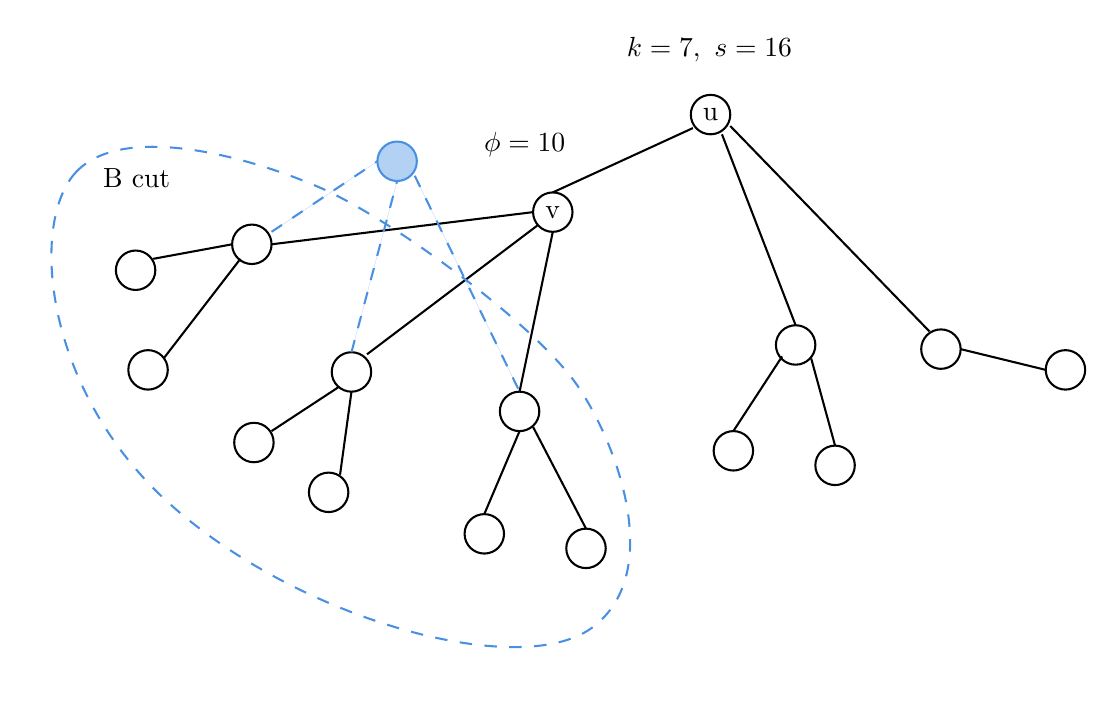
\begin{tikzpicture}[x=0.75pt,y=0.75pt,yscale=-1,xscale=1]
%uncomment if require: \path (0,471); %set diagram left start at 0, and has height of 471

%Shape: Circle [id:dp34076887970340053]
\draw  [fill={rgb, 255:red, 255; green, 255; blue, 255 }  ,fill opacity=1 ] (392,61.5) .. controls (392,56.25) and (396.25,52) .. (401.5,52) .. controls (406.75,52) and (411,56.25) .. (411,61.5) .. controls (411,66.75) and (406.75,71) .. (401.5,71) .. controls (396.25,71) and (392,66.75) .. (392,61.5) -- cycle ;

%Shape: Circle [id:dp9085081530378656]
\draw  [fill={rgb, 255:red, 255; green, 255; blue, 255 }  ,fill opacity=1 ] (316,108.5) .. controls (316,103.25) and (320.25,99) .. (325.5,99) .. controls (330.75,99) and (335,103.25) .. (335,108.5) .. controls (335,113.75) and (330.75,118) .. (325.5,118) .. controls (320.25,118) and (316,113.75) .. (316,108.5) -- cycle ;

%Shape: Circle [id:dp40613127689805917]
\draw  [fill={rgb, 255:red, 255; green, 255; blue, 255 }  ,fill opacity=1 ] (403,223.5) .. controls (403,218.25) and (407.25,214) .. (412.5,214) .. controls (417.75,214) and (422,218.25) .. (422,223.5) .. controls (422,228.75) and (417.75,233) .. (412.5,233) .. controls (407.25,233) and (403,228.75) .. (403,223.5) -- cycle ;
%Shape: Circle [id:dp9931876018636179]
\draw  [fill={rgb, 255:red, 255; green, 255; blue, 255 }  ,fill opacity=1 ] (503,174.5) .. controls (503,169.25) and (507.25,165) .. (512.5,165) .. controls (517.75,165) and (522,169.25) .. (522,174.5) .. controls (522,179.75) and (517.75,184) .. (512.5,184) .. controls (507.25,184) and (503,179.75) .. (503,174.5) -- cycle ;
%Shape: Circle [id:dp7698586857134941]
\draw  [fill={rgb, 255:red, 255; green, 255; blue, 255 }  ,fill opacity=1 ] (563,184.5) .. controls (563,179.25) and (567.25,175) .. (572.5,175) .. controls (577.75,175) and (582,179.25) .. (582,184.5) .. controls (582,189.75) and (577.75,194) .. (572.5,194) .. controls (567.25,194) and (563,189.75) .. (563,184.5) -- cycle ;
%Shape: Circle [id:dp07661905351809639]
\draw  [fill={rgb, 255:red, 255; green, 255; blue, 255 }  ,fill opacity=1 ] (452,230.5) .. controls (452,225.25) and (456.25,221) .. (461.5,221) .. controls (466.75,221) and (471,225.25) .. (471,230.5) .. controls (471,235.75) and (466.75,240) .. (461.5,240) .. controls (456.25,240) and (452,235.75) .. (452,230.5) -- cycle ;
%Shape: Circle [id:dp6823852359253104]
\draw  [fill={rgb, 255:red, 255; green, 255; blue, 255 }  ,fill opacity=1 ] (433,172.5) .. controls (433,167.25) and (437.25,163) .. (442.5,163) .. controls (447.75,163) and (452,167.25) .. (452,172.5) .. controls (452,177.75) and (447.75,182) .. (442.5,182) .. controls (437.25,182) and (433,177.75) .. (433,172.5) -- cycle ;
%Straight Lines [id:da2795330732074286]
\draw    (407,71) -- (442.5,163) ;


%Straight Lines [id:da95361289139327]
\draw    (411,67) -- (507,166) ;


%Straight Lines [id:da03919277897290474]
\draw    (436,178) -- (412.5,214) ;


%Straight Lines [id:da6790046753307697]
\draw    (450,179) -- (461.5,221) ;


%Straight Lines [id:da3674173158335614]
\draw    (563,184.5) -- (522,174.5) ;


%Straight Lines [id:da02933874590346841]
\draw    (393,68) -- (325.5,99) ;


%Shape: Circle [id:dp6930911043272474]
\draw  [fill={rgb, 255:red, 255; green, 255; blue, 255 }  ,fill opacity=1 ] (172,219.5) .. controls (172,214.25) and (176.25,210) .. (181.5,210) .. controls (186.75,210) and (191,214.25) .. (191,219.5) .. controls (191,224.75) and (186.75,229) .. (181.5,229) .. controls (176.25,229) and (172,224.75) .. (172,219.5) -- cycle ;
%Shape: Circle [id:dp4545176452788231]
\draw  [fill={rgb, 255:red, 255; green, 255; blue, 255 }  ,fill opacity=1 ] (208,243.5) .. controls (208,238.25) and (212.25,234) .. (217.5,234) .. controls (222.75,234) and (227,238.25) .. (227,243.5) .. controls (227,248.75) and (222.75,253) .. (217.5,253) .. controls (212.25,253) and (208,248.75) .. (208,243.5) -- cycle ;
%Shape: Circle [id:dp030374617759524325]
\draw  [fill={rgb, 255:red, 255; green, 255; blue, 255 }  ,fill opacity=1 ] (219,185.5) .. controls (219,180.25) and (223.25,176) .. (228.5,176) .. controls (233.75,176) and (238,180.25) .. (238,185.5) .. controls (238,190.75) and (233.75,195) .. (228.5,195) .. controls (223.25,195) and (219,190.75) .. (219,185.5) -- cycle ;
%Straight Lines [id:da016875084395338025]
\draw    (222,193) -- (190,214) ;


%Straight Lines [id:da7587321706433352]
\draw    (228.5,195) -- (223,235) ;


%Shape: Circle [id:dp6805190369347967]
\draw  [fill={rgb, 255:red, 255; green, 255; blue, 255 }  ,fill opacity=1 ] (283,263.5) .. controls (283,258.25) and (287.25,254) .. (292.5,254) .. controls (297.75,254) and (302,258.25) .. (302,263.5) .. controls (302,268.75) and (297.75,273) .. (292.5,273) .. controls (287.25,273) and (283,268.75) .. (283,263.5) -- cycle ;
%Shape: Circle [id:dp49294006336897334]
\draw  [fill={rgb, 255:red, 255; green, 255; blue, 255 }  ,fill opacity=1 ] (332,270.5) .. controls (332,265.25) and (336.25,261) .. (341.5,261) .. controls (346.75,261) and (351,265.25) .. (351,270.5) .. controls (351,275.75) and (346.75,280) .. (341.5,280) .. controls (336.25,280) and (332,275.75) .. (332,270.5) -- cycle ;
%Shape: Circle [id:dp4780933458297658]
\draw  [fill={rgb, 255:red, 255; green, 255; blue, 255 }  ,fill opacity=1 ] (300,204.5) .. controls (300,199.25) and (304.25,195) .. (309.5,195) .. controls (314.75,195) and (319,199.25) .. (319,204.5) .. controls (319,209.75) and (314.75,214) .. (309.5,214) .. controls (304.25,214) and (300,209.75) .. (300,204.5) -- cycle ;
%Straight Lines [id:da9579747847325664]
\draw    (309.5,214) -- (292.5,254) ;


%Straight Lines [id:da24682160488454663]
\draw    (316,212) -- (341.5,261) ;


%Straight Lines [id:da7254371683892009]
\draw    (318,115) -- (236,177) ;


%Straight Lines [id:da9361718285942648]
\draw    (325.5,118) -- (309.5,195) ;


%Shape: Circle [id:dp7136610740709559]
\draw  [fill={rgb, 255:red, 255; green, 255; blue, 255 }  ,fill opacity=1 ] (171,124) .. controls (171,118.75) and (175.25,114.5) .. (180.5,114.5) .. controls (185.75,114.5) and (190,118.75) .. (190,124) .. controls (190,129.25) and (185.75,133.5) .. (180.5,133.5) .. controls (175.25,133.5) and (171,129.25) .. (171,124) -- cycle ;
%Shape: Circle [id:dp7986023789770009]
\draw  [fill={rgb, 255:red, 255; green, 255; blue, 255 }  ,fill opacity=1 ] (115,136.5) .. controls (115,131.25) and (119.25,127) .. (124.5,127) .. controls (129.75,127) and (134,131.25) .. (134,136.5) .. controls (134,141.75) and (129.75,146) .. (124.5,146) .. controls (119.25,146) and (115,141.75) .. (115,136.5) -- cycle ;
%Straight Lines [id:da8486079993175883]
\draw    (316,108.5) -- (190,124) ;


%Straight Lines [id:da27547813733695325]
\draw    (171,124) -- (133,131) ;


%Shape: Circle [id:dp08981252883235546]
\draw  [fill={rgb, 255:red, 255; green, 255; blue, 255 }  ,fill opacity=1 ] (121,184.5) .. controls (121,179.25) and (125.25,175) .. (130.5,175) .. controls (135.75,175) and (140,179.25) .. (140,184.5) .. controls (140,189.75) and (135.75,194) .. (130.5,194) .. controls (125.25,194) and (121,189.75) .. (121,184.5) -- cycle ;
%Straight Lines [id:da22823959276419536]
\draw    (175,131) -- (138,179) ;


%Shape: Polygon Curved [id:ds15408437148876897]
\draw  [color={rgb, 255:red, 74; green, 144; blue, 226 }  ,draw opacity=1 ][dash pattern={on 4.5pt off 4.5pt}] (96,89) .. controls (119,65) and (180,82) .. (214,97) .. controls (248,112) and (318,163) .. (338,193) .. controls (358,223) and (379,284) .. (344,309) .. controls (309,334) and (204,305) .. (142,250) .. controls (80,195) and (73,113) .. (96,89) -- cycle ;
%Shape: Circle [id:dp5861650780323242]
\draw  [color={rgb, 255:red, 74; green, 144; blue, 226 }  ,draw opacity=1 ][fill={rgb, 255:red, 179; green, 209; blue, 243 }  ,fill opacity=1 ] (241,84) .. controls (241,78.75) and (245.25,74.5) .. (250.5,74.5) .. controls (255.75,74.5) and (260,78.75) .. (260,84) .. controls (260,89.25) and (255.75,93.5) .. (250.5,93.5) .. controls (245.25,93.5) and (241,89.25) .. (241,84) -- cycle ;
%Straight Lines [id:da880896354333569]
\draw [color={rgb, 255:red, 74; green, 144; blue, 226 }  ,draw opacity=1 ][fill={rgb, 255:red, 74; green, 144; blue, 226 }  ,fill opacity=1 ] [dash pattern={on 4.5pt off 4.5pt}]  (190,118) -- (241,84) ;


%Straight Lines [id:da2721999945811009]
\draw [color={rgb, 255:red, 74; green, 144; blue, 226 }  ,draw opacity=1 ][fill={rgb, 255:red, 74; green, 144; blue, 226 }  ,fill opacity=1 ] [dash pattern={on 4.5pt off 4.5pt}]  (228.5,176) -- (250.5,93.5) ;


%Straight Lines [id:da9627189828730469]
\draw [color={rgb, 255:red, 74; green, 144; blue, 226 }  ,draw opacity=1 ][fill={rgb, 255:red, 74; green, 144; blue, 226 }  ,fill opacity=1 ] [dash pattern={on 4.5pt off 4.5pt}]  (259,91) -- (309.5,195) ;



% Text Node
\draw (401.5,61.5) node  [align=left] {u};
% Text Node
\draw (325.5,108.5) node  [align=left] {v};
% Text Node
\draw (312,76) node  [align=left] {$\displaystyle \phi =10$};
% Text Node
\draw (401,30) node [color={rgb, 255:red, 0; green, 0; blue, 0 }  ,opacity=1 ] [align=left] {$\displaystyle k=7,\ s=16$};
% Text Node
\draw (125,92) node  [align=left] {B cut};


\end{tikzpicture}

	\caption{Example decompose step}
	\label{fig:decompose_example}
\end{figure}

The component size is \(s=16\), and the anonymization parameter is \(k=7\). \(s \ge max\{2k-1,3k-5\}=max\{13,16\}\) is true, so the component is considered oversized and needs to be cut. The root of the largest sized subtree is \textit{v}, and its size is \(\phi=10\).

Since \(s-\phi \ge k-1\), we can proceed with one of the cut types. In fact, in this case \(s-\phi=k-1=6\), so we will need to apply cut type B as highlighted by the dotted line in figure \ref{fig:decompose_example}.

In order to keep the nodes in the cut partition together, we insert a \emph{Steiner's Vertex}. This vertex is also highlighted on figure \ref{fig:decompose_example} with dotted edges.

The resulting two partitions are of size 7 and 9 -- note, that the \emph{Steiner's Vertex} does not count into the component's size. Both partitions are of proper size now.

\subsection{Polynomial-time approximation algorithm}

\paragraph{Theorem}  There is a polynomial-time algorithm for the k-Anonymity problem, that achieves an approximation ratio of \(max\{2k-1, 3k-5\}\). \cite{aggarwal}

\paragraph{Proof} First, use algorithm \textsc{Forest} to create a forest with cost at most OPT and minimum tree size at least \textit{k}. Then repeatedly apply algorithm \textsc{Decompose component} to any component that has size larger than \(max\{2k-1, 3k-5\}\). Note that both these algorithms terminate in \(\mathcal{O}(kn^2)\) time. \cite{aggarwal}

\section{Summary}

As we have seen in this chapter, it is possible to give a polynomial-time approximation algorithm for the k-anonymity with generalization problem, and the algorithm gives an approximation ratio of \(max\{2k-1, 3k-5\}\).

We have started by defining the input table as a set of row vectors, and transforming the input data into its graph representation. We have discussed the limitations of the graph representation, and why we can only achieve an \(\mathcal{O}(k)\) approximation.

Next we have introduced the three main steps in the algorithm: cost-graph calculation, the \textsc{Forest building} algorithm, and the \textsc{Decompose component} algorithm. We have introduced each of them in great detail with examples, and finally have proven that the polynomial-time approximation algorithm exists by giving its formalized description.

In the next chapter we will introduce a software library written in the Go programming language by the author, which implements the approximation algorithm discussed in this chapter.